\subsection{Observed TCEs}

\label{s:tces}
As with the previous three Kepler planet candidate catalogs \citep{Coughlin2016,Mullally2015cat,Rowe2015cat}, the population of events that were used to create KOIs and planet candidates are known as \opstce s. These are periodic reductions of flux in the light curve that were found by the TPS module and evaluated by the DV module of the \Kepler{} Pipeline \citep{JenkinsKDPH} \footnote{The source code of the entire Pipeline is available at \url{https://github.com/nasa/kepler-pipeline}}. The Data Release 25 \opstce{s}  were created by running the SOC 9.3 version of the \Kepler\ Pipeline on the DR25, Q1--Q17 \Kepler\ PDC time-series.  For a thorough discussion of the DR25 TCEs and on the pipeline's search see \citet{Twicken2016}. 

The DR25 \opstce s, their ephemerides, and the metrics calculated by the pipeline are available at the NASA Exoplanet Archive \citep{Akeson2013}.  In this paper we endeavor to disposition these signals into planet candidates and false positives.  Because the \opstce s act as the input to our catalog, we first describe some of their properties as a whole and reflect on how they are different from the \opstce{} populations found with previous searches.

We have plotted the distribution of the \ntcesnorogue\ \opstce s in terms of period in Figure~\ref{f:obstces}. Notice that there is an excessive number of short and long period \opstce{s} compared to the number of expected transiting planets. Not shown, but worth noting is that the number of \opstce{s} increases with decreasing MES.

As with previous catalogs, the short period ($<10$\,d) excess is dominated by true variability of stars due to both intrinsic stellar variability (e.g., spots or pulsations) and contact/near-contact eclipsing binaries. The long period excess is dominated by instrumental noise. For example, a decrease in flux following a cosmic ray hit (known as an SPSD \citep{KDCH}), can match up with other decrements in flux to produce a TCE. Also, image artifacts known as rolling-bands are very strong on some channels \citep[see \S6.7 of][]{KIH}  and since the spacecraft rolls approximately every 90\,d, causing a star to move on/off a \Kepler\ detector with significant rolling band noise, these variations can easily line up to produce TCEs at \Kepler{'s} heliocentric orbital period ($\approx$372 days, 2.57 in log-space). This is the reason for the largest spike in the \opstce\ population seen in Figure~\ref{f:obstces}. The narrow spike at 459 days (2.66 in log-space) in the DR24 \opstce{} distribution is caused by edge-effects near three equally spaced data gaps in the DR24 data processing.  The short period spikes in the distribution of both the DR25 and DR24 \opstce{s} is caused by contamination by bright variable stars (see \S\ref{s:ephemmatch} and \citet{Coughlin2014}).

Generally, the excess of long period TCEs is significantly larger than it was in the DR24 TCE catalog \citep{Seader2015}, also seen in Figure~\ref{f:obstces}. Most likely, this is because DR24 implemented an aggressive veto known as the bootstrap metric \citep{Seader2015}.  For DR25 this metric was calculated, but was not used as a veto. Also, other vetoes were made less strict causing more TCEs across all periods to be created. 

To summarize, for DR25 the number of false signals among the \opstce{s}  is dramatically larger than in any previous catalog. This was done on purpose in order to increase the Pipeline completeness and more transiting exoplanets to be made into \opstce{s}. 

\begin{figure*}[ht]
 \begin{center}
  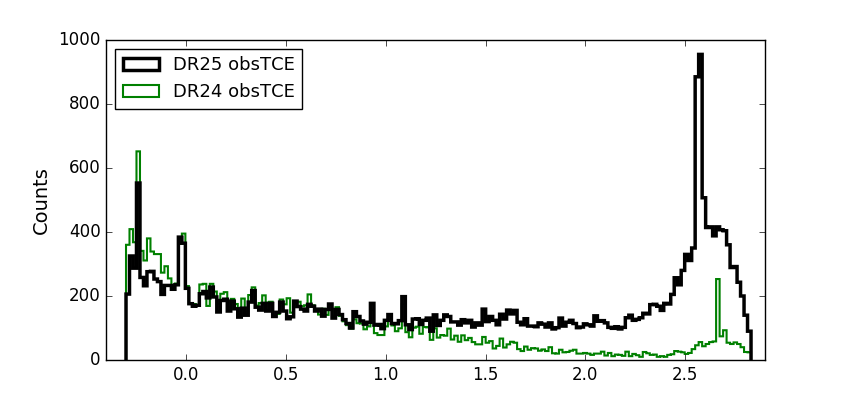
\includegraphics[width=0.85\linewidth]{fig-obstcePeriods.png}
  \caption{Histogram of the log$_{10}$(period) in days of the DR25 \opstce{s} (black). The DR24 catalog obsTCEs \citep{Seader2015} are shown in green for comparison. The number of long-period TCEs is much larger for DR25 and includes a large spike in the number of TCEs at the orbital period of the spacecraft (372 days, or 2.57 in log-space). The long and short period spikes for both distributions are discussed in \S\ref{s:tces}.}
  %\caption{\ref{f:tces} A two dimensional histogram of the number of TCEs by log(period) and log(MES). The marginalized distributions for log(period) and log(MES) are projected along their respective axes and shown on the top and right respectively. }
  \label{f:obstces} 
 \end{center}
 \end{figure*}



\subsection{Rogue TCEs}
The DR25 TCE table at the NASA Exoplanet Archive contains \ntcesnorogue\ \opstce{s} and 1498 rogue TCEs \footnote{See the tce\_rogue\_flag column in the DR25 TCE table at the exoplanet archive.} for a total of \ntces. The rogue TCEs were created because of a bug in the Kepler pipeline which let through certain three-transit events.  This bug was not in place when characterizing the Pipeline using flux-level transit injection \citep[see][]{Burke2017a,Burke2017b} and because the primary purpose of this catalog is to be able to accurately calculate occurrence rates, we do not use the rogue TCEs in the creation and analysis of the DR25 KOI catalog. Also note that all of the TCE populations (observed, injection, inversion and scrambling, see the next section) had rogue TCEs that were removed prior to analysis. The creation and analysis of this KOI catalog only rely on the non-rogue TCEs. 

